\section{Modello per Object Detection}

L'obiettivo del lavoro è quello di effettuare detection sui rifiuti plastici
su immagini e per questo si è optato su una architettura basata su rete convoluzionale che allo stato dell'arte sia efficacie e abbia anche 
facilità nell'utilizzo. La scelta è ricaduta su YOLO, You Only Look Once, in
quanto risulta una delle architetture più utilizzate ed performanti.
A maggior ragione, il dataset a nostra disposizione era già predisposto per 
essere compatibile con YOLO.

Ci siamo basati sulla libreria YOLO di \href{https://docs.ultralytics.com/}{ultralytics} in quanto possiede molti metodi e strumenti per lavorare al meglio con il modello. In particolare molto utile la gestione interna per 
fare augmentation direttamente durante la fase di training.

All'inizio del progetto era a disposizione la versione 8 di YOLO che è stata
poi la versione da noi utilizzata sebbene in questi ultimi mesi sono state 
presentate le versioni 9 e 10. Abbiamo preferito mantenere per continuità con il lavoro la versione 8, che di recente ha visto anche l'aggiornamento
alla versione 8.2, una versione che mantiene la stessa struttura per quanto
riguarda l'architettura ma ha performance migliori.



\subsection*{Architettura di YOLOv8}

L'architettura di YOLOv8 si basa su un approccio end-to-end che suddivide l'immagine in una griglia e applica convoluzioni multiple per predire le bounding box e le classi degli oggetti all'interno di ciascuna cella della griglia. YOLOv8 utilizza tecniche avanzate come la \textit{Path Aggregation Network} (PANet) per migliorare l'integrazione delle informazioni a diversi livelli di profondità della rete, il che è fondamentale per rilevare oggetti di varie dimensioni e scale. Nella figura \ref*{fig:2} è riportato un diagramma semplificato dell'architettura.

\begin{figure}[h!]
    \centering
    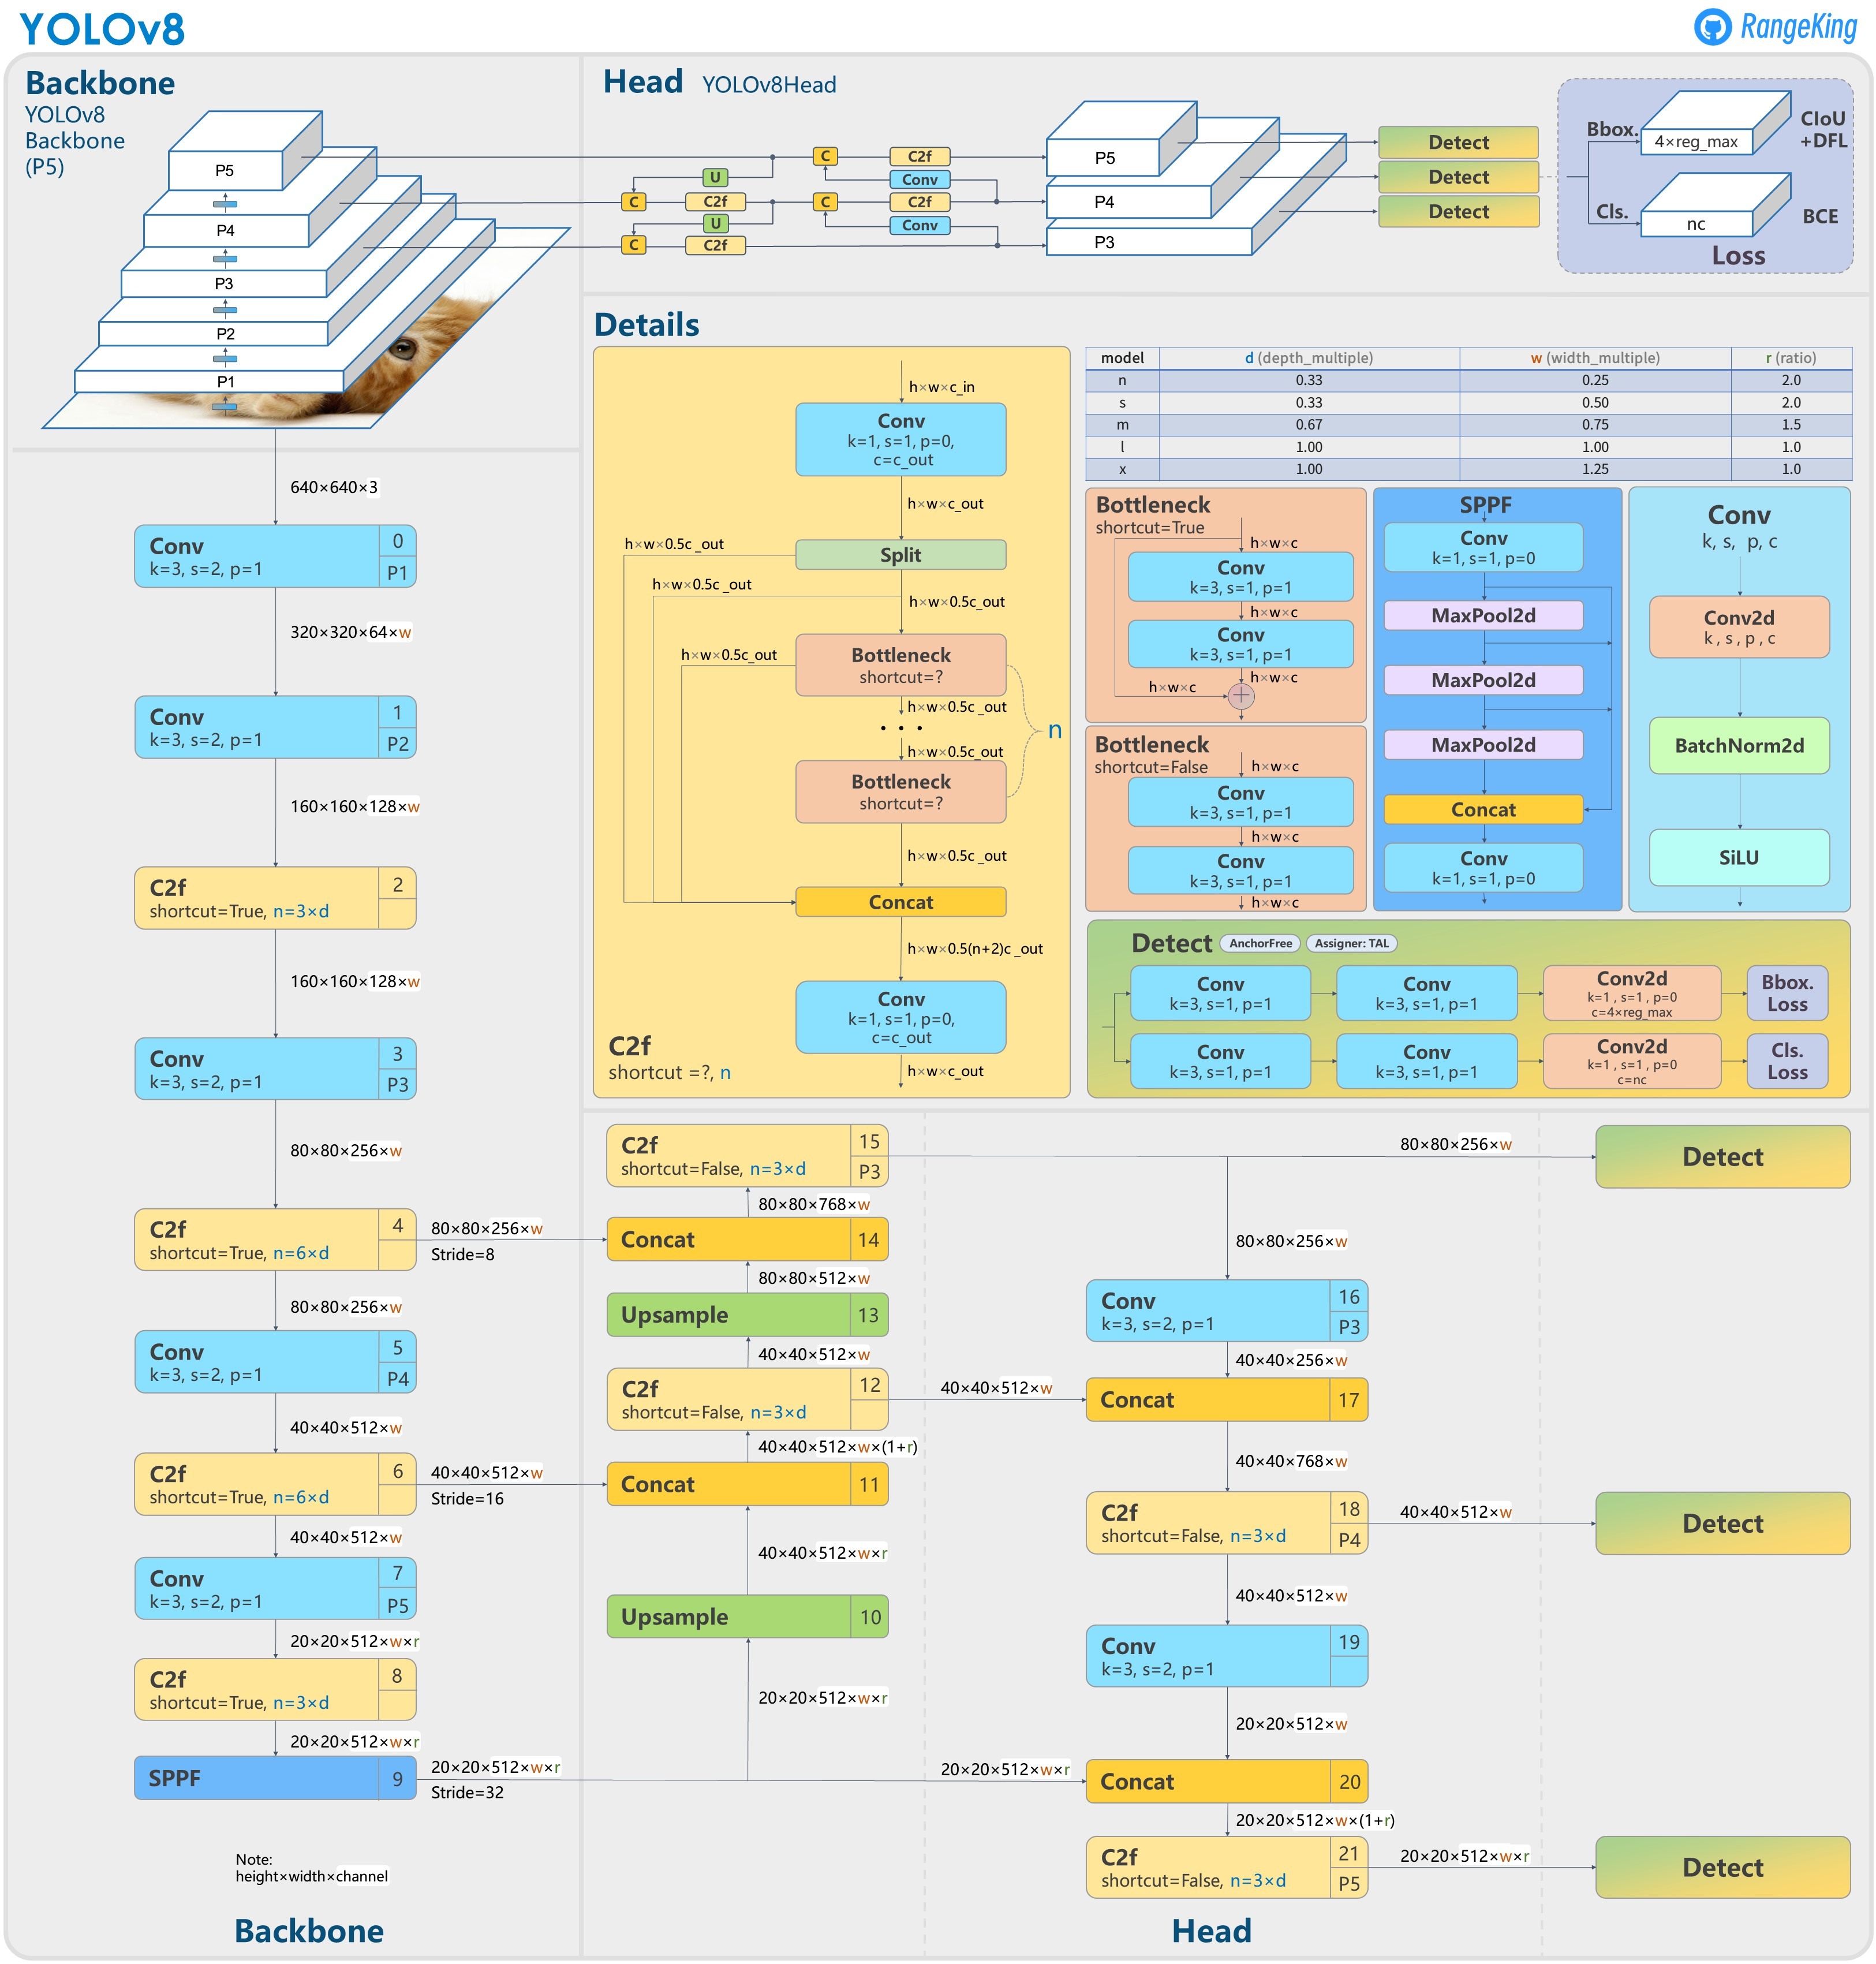
\includegraphics[width=\textwidth]{yolov8_architecture.jpg}
    \caption{Schema dell'architettura di YOLOv8}
    \label{fig:2}
\end{figure}

Il modello YOLOv8 incorpora anche una \textit{Neck} e una \textit{Head} ottimizzati per massimizzare la capacità di rilevamento attraverso una migliore aggregazione delle caratteristiche e una maggiore flessibilità nelle predizioni finali. L'uso di meccanismi come le \textit{Depthwise Separable Convolutions} contribuisce a ridurre il numero di operazioni computazionali, mantenendo un'elevata capacità espressiva del modello.

\subsection*{Dimensioni delle architetture usate}

Nell'ambito del progetto, si è scelto di utilizzare le varianti \textbf{small}, \textbf{medium} e \textbf{nano} di YOLOv8 per il task di object detection, in quanto queste architetture offrono un buon compromesso tra capacità computazionale e performance, risultando particolarmente adatte per l'esecuzione su hardware con risorse limitate quali quelle a noi disponibili.

\subsection*{Vantaggi di YOLOv8 per il Riconoscimento dei Rifiuti Plastici}

La scelta di YOLOv8 per il riconoscimento dei rifiuti plastici nei fiumi è giustificata da diversi fattori:

\begin{itemize}
    \item \textbf{Rilevamento in Tempo Reale}: YOLOv8 è noto per la sua capacità di eseguire object detection in tempo reale, il che è cruciale per applicazioni di monitoraggio continuo nei fiumi. La possibilità di rilevare e classificare i rifiuti plastici in tempo reale consente interventi immediati, riducendo il rischio che i rifiuti possano propagarsi ulteriormente.
    
    \item \textbf{Efficienza Computazionale}: Le versioni di YOLO sono ottimizzate per girare su hardware con risorse limitate, come droni o sistemi embedded. Questo le rende particolarmente adatte per applicazioni sul campo, dove la potenza di calcolo potrebbe essere un vincolo.
    
    \item \textbf{Accuratezza Elevata}: Nonostante la sua velocità, YOLOv8 mantiene un'accuratezza competitiva grazie all'uso di tecniche avanzate come l'addestramento con \textit{label smoothing} e l'adozione di una griglia più fine per la previsione delle bounding box. Questo è essenziale per distinguere efficacemente i rifiuti plastici da altri detriti naturali presenti nei fiumi, come è possibile vedere in un esempio alla figura \ref*{fig:3}.
\end{itemize}

\begin{figure}[h!]
    \centering
    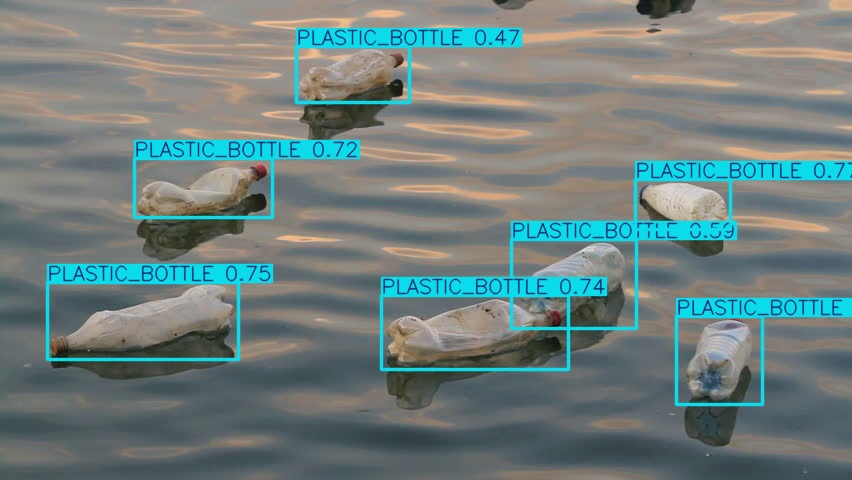
\includegraphics[width=\textwidth]{res_1203_1.jpg} 
    \caption{Esempio di output di YOLOv8 per il rilevamento di rifiuti plastici nei fiumi.}
    \label{fig:3}
\end{figure}
